%%%%%%%%%%%%%%%%%%%%%%%%%%%%%%%%%%%%%%%%%%%%%%%%%%%%%%%%%%%%%%%%%%%%%%%%%%%%%%%
%%                                                                           %%
%%   Dr Todd R Jones, Dr Luis Patino, Dr Lily Sun                            %%
%%   Department of Computer Science
%% 
%%   University of Reading, UK                                               %%
%%                                                                           %%
%%  Based on template created by Dr Varun Ojha                               %%
%%                                                                           %%
%%%%%%%%%%%%%%%%%%%%%%%%%%%%%%%%%%%%%%%%%%%%%%%%%%%%%%%%%%%%%%%%%%%%%%%%%%%%%%%
%%%%     SETTING STARTS - DO NOT CHANGE Unless your TeX setting require so   %%
%%%%%%%%%%%%%%%%%%%%%%%%%%%%%%%%%%%%%%%%%%%%%%%%%%%%%%%%%%%%%%%%%%%%%%%%%%%%%%%
%%----------------------------------------------------------------------------------
% DO NOT Change this. It is the required setting A4 page, 11pt, onside print, book style
%%----------------------------------------------------------------------------------
\documentclass[a4paper,11pt,oneside]{book}
\usepackage{CS_report} % DO NOT REMOVE THIS LINE. 
\usepackage{natbib} % Added for citation commands
%%%%%%%%%%%%%%%%%%%%%%%%%%%%%%%%%%%%%%%%%%%%%%%%%%%%%%%%%%%%%%%%%%%%%%%%%%%%%%%%%%%%%%%


%%%%%%%%%%%%%%%%%%%%%%%%%%%%%%%%%%%%%%%%%%%%%%%%%%%%%%%%%%%%%%%%%%%%%%%%%%%%%%%%%%%%%%%
\begin{document}

    \captionsetup[figure]{margin=1.5cm,font=small,name={Figure},labelsep=colon}
    \captionsetup[table]{margin=1.5cm,font=small,name={Table},labelsep=colon}
    
    \frontmatter
    
    \begin{titlepage}      
        \begin{center}
            
\includegraphics[width=3cm]{figures/uorlogo.png}\\[0.5cm]
            {\LARGE University of Reading\\[0.5cm]
            Department of Computer Science}\\[2cm]
			%{\color{blue} \rule{\textwidth}{1pt}}
			
			% -------------------------------
			% You need to edit some details here
			% -------------------------------  
            \linespread{1.2}\huge {
                %%%%%%%%%%%%%%%%%%%%%%%%%%%%
                %TODO: 1 TITLE of Your PROJECT 
                %%%%%%%%%%%%%%%%%%%%%%%%%%%%
                % change the following line                
                Routers for LLM: A Framework for Model Selection and Tool Invocation
            
            }
            \linespread{1}~\\[2cm]
			%{\color{blue} \rule{\textwidth}{1pt}}
            {\Large 
                %%%%%%%%%%%%%%%%%%%%%%%%%%%%
                %TODO: 2 YOUR NAME
                %%%%%%%%%%%%%%%%%%%%%%%%%%%%             
                % change the following line
                Ruben J. Lopes
                % change end             
            }\\[1cm] 
            

            {\large 
                %%%%%%%%%%%%%%%%%%%%%%%%%%%%
                %TODO: 3 YOUR NAME Supervisor's name(s)
                %%%%%%%%%%%%%%%%%%%%%%%%%%%%             
                % change the following line                
                \emph{Supervisor:} Dr. Xiaomin Chen}\\[1cm] % if applicable

                %%%%%%%%%%%%%%%%%%%%%%%%%%%%
    		% TODO: Verify that degree names are correct %
                %%%%%%%%%%%%%%%%%%%%%%%%%%%%
            \large A report submitted in partial fulfilment of the requirements of\\the University of Reading for the degree of\\ Bachelor of Science in \textit{Computer Science}\\[0.3cm] 
            \vfill
            
            
            \today % Please update this date you can use \date{April 2020} for fixed date
        \end{center}
    \end{titlepage}
    
    
    % -------------------------------------------------------------------
    % Declaration
    % -------------------------------------------------------------------
    \newpage
    \thispagestyle{empty}
    \chapter*{\Large Declaration}
    % PLEASE CHANGE THIS TEXT EXCEPT YOUR NAME%
    % -------------------------------
    %TODO: PLEASE ONLY UPDATE HERE -- PLEASE WRITE YOUR NAME %    
    % ------------------------------- 
    I,
    %%%%%%%%%%%%%%%%%%%%%%%
    Ruben J. Lopes
    %%%%%%%%%%%%%%%%%%%%%%%
    of the Department of Computer Science, University of Reading, confirm that this is my own work and figures, tables, equations, code snippets, artworks, and illustrations in this report are original and have not been taken from any other person's work, except where the works of others have been explicitly acknowledged, quoted, and referenced. I understand that if failing to do so will be considered a case of plagiarism. Plagiarism is a form of academic misconduct and will be penalised accordingly. \\
    
    %% Please delete as appropriate. 
    \noindent
    %%%%%%%%%%%%%%%%%%%%%%%%%%%%%%%%%%%%%%%%%%%%%%% 
    %TODO 1 Consent for example copy -  we will use 
    I give consent to a copy of my report being shared with future students as an exemplar. \\
    
    \noindent
    %%%%%%%%%%%%%%%%%%%%%%%%%%%%%%%%%%%%%%%%%%%%%%% 
    %TODO 2 Consent to let the report to use use by library for public use
    I give consent for my work to be made available more widely to members of UoR and public with interest in teaching, learning and research. 
    %%%%%%%%%%%%%%%%%%%%%%%%%%%%%%%%%%%%%%%%%%%%%%%
    ~\\[1cm]
    \begin{flushright}
	%------------------------------ 
	% change the following line
    %TODO: PLEASE UPDATE  Your Name  -------------------------------%
	Ruben J. Lopes\\
    
    \today
    \end{flushright}

     
    % -------------------------------------------------------------------
    % Abstract and Acknowledgement
    % -------------------------------------------------------------------
    
    \chapter*{\center \Large  Abstract}

\noindent In the current landscape of large language models, users are confronted with a plethora of models and tools each offering a unique blend of specialisation and generality. This project proposes the development of a dynamic middleware \textit{router} designed to automatically assign user queries to the most appropriate model or tool within a multi agent system. By using zero shot Natural Language Inference models, the router will evaluate incoming prompts against criteria such as task specificity and computational efficiency, and \textit{route} the prompt to the most effective model and/or allow specific tools relevant that the model could use.

The proposed framework is underpinned by three core routing mechanisms:

\begin{itemize}
    \item Firstly, it will direct queries to cost effective yet sufficiently capable models, a concept that builds on existing work in semantic routing \cite{ong2025routellmlearningroutellms}.
    
    \item Secondly, it incorporates a tool routing system that automatic invocation of specialised functions, thus streamlining user interaction and reducing inefficiencies currently inherent in systems like OpenAI's and Open Web UI. Furthermore this could also reduce inefficiencies in the recent reasoning models addressing the observed dichotomy between underthinking with complex prompts and overthinking with simpler queries when reasoning is manually toggled which can be costly and could cause hallucination.
    
    \item Thirdly, while the primary focus remains on model and tool routing, this work will preliminarily explore the potential application of the routing architecture as a security mechanism. Initial investigations will examine the theoretical feasibility of leveraging the router's natural language understanding capabilities to identify adversarial prompts. This includes a preliminary assessment of detection capabilities for prompt engineering attempts, potential jailbreaking patterns, and anomalous tool usage requests. However, given the rapidly evolving nature of LLM security threats and the complexity of implementing robust safeguards, comprehensive security features remain outside the core scope of this research. Although this aspect represents a promising direction for potential future work, particularly as the field of LLM security continues to grow.
\end{itemize}

\noindent By integrating these mechanisms, the research aims to pioneer a more efficient, modular, and secure distributed AI architecture. This architecture not only optimises resource allocation but also reinforces system integrity against emerging adversarial threats, thereby contributing novel insights into the development of next generation LLM deployment strategies.
    % -------------------------------------------------------------------
	% Acknowledgement
	% -------------------------------------------------------------------
   
    \chapter*{\center \Large  Acknowledgements}
%%%% Update with your text %%%%%%%%%%%%%%%
An acknowledgements section is optional. You may like to acknowledge the support and help of your supervisor(s), friends, or any other person(s), department(s), institute(s), etc. If you have been provided specific facility from department/school acknowledged so.  

   
    
    % -------------------------------------------------------------------
    % Contents, list of figures, list of tables
    % -------------------------------------------------------------------
    
    \tableofcontents
    \listoffigures
    \listoftables
    \chapter*{List of Abbreviations}
\chaptermark{List of Abbreviations}
%%%%%%%%%%%%%%%%%%%%%%%%%%%%%%%%%%%
%%  Enter your list of Abbreviation and Symbols in this file
%%%%%%%%%%%%%%%%%%%%%%%%%%%%%%%%%%%
\begin{abbrv}
    
    \item[SMPCS]			School of Mathematical, Physical and Computational Sciences
    
\end{abbrv}
 %  Enter your list of Abbreviation and Symbols in this file
    
    %%%%%%%%%%%%%%%%%%%%%%%%%%%%%%%%%%%%%%%%%%%%%%%%%%%%%%%%%%%%%%%%%%%%%%%%
    %%                                                                    %%  
    %%  Main chapters and sections of your project                        %%  
    %%  Everything from here on needs updates in your own words and works %%
    %%                                                                    %%
    %%%%%%%%%%%%%%%%%%%%%%%%%%%%%%%%%%%%%%%%%%%%%%%%%%%%%%%%%%%%%%%%%%%%%%%%
    \mainmatter
    % Read for preparation of document in LaTex 
    % Lamport, L. (1986), LATEX: A Document Preparation System, Addison-Wesley.
    
    \chapter{Introduction}
\label{ch:into}

In the past few years the landscape of large language models has expanded dramatically, with many domain specific as well as general-purpose agents emerging across domains such as healthcare (like Med-PaLM 2 and BioGPT), coding (like CodeLlama and GitHub Copilot), and research (like Claude Opus and GPT-4o). Organisations that provide inference as a service now face complex trade-offs between cost, latency, and capability: for example, GPT-4.5 can cost up to \$75 per million tokens compared with just \$0.15 for gemini-2.5-flash\footnote{https://sanand0.github.io/llmpricing/}\footnote{https://artificialanalysis.ai/}. Although these models could be vastly different in terms of capability, the problem organisations face is determining \textit{when} to deploy premium models versus more cost-effective alternatives for a given task / prompt. This suggests a need for intelligent routing systems that can analyse incoming prompts and direct them to the most appropriate model based on task complexity, required capabilities, and cost considerations.

Inspired by lower level (transformer-embedded) "router" such as the one employed by mistral for their Mixtral (MoE) model the goal of this was to allow for a more distributed, higher level prompt based routing between a verity of models with varying levels of cost and complexity.

%%%%%%%%%%%%%%%%%%%%%%%%%%%%%%%%%%%%%%%%%%%%%%%%%%%%%%%%%%%%%%%%%%%%%%%%%%%%%%%%%%%
\section{Problem statement}
\label{sec:intro_prob_art}

The proliferation of large language models has created a complex ecosystem where selecting the optimal model for a given task has become increasingly challenging.

Existing multi-agent routing systems reveal several shortcomings. First, many current routers rely on \textbf{manual configuration}. For example, Both Open AI's as well as Open WebUI's chat interface require explicitly toggling of tools/selection of agents from users, and listing models to skip, on a per-chat basis. This manual toggling is brittle. Second, LLM-based routers can suffer from reasoning \textbf{inefficiencies}. Recent studies identify \textit{"underthinking"} (prematurely abandoning good reasoning paths) and \textit{"overthinking"} (generating excessive, unnecessary steps) in modern LLMs. For instance, Wang \textit{et al.} (2025) find that top reasoning models often switch thoughts too quickly – an \textit{"underthinking"} effect that hurts accuracy\footnote{https://arxiv.org/pdf/2501.18585v1}. Conversely, Kumar \textit{et al.} demonstrate how even simple queries can be made to "overthink" (spending many tokens on irrelevant chains of thought) without improving answers\footnote{https://arxiv.org/pdf/2502.02542v1}. Both phenomena imply wasted tokens. Finally, prompt interpretation remains imperfect: ambiguous or poorly phrased queries may be misrouted or require multiple LLM calls to resolve intent, leading to inefficiency.

Organisations and users face several key problems:
\begin{enumerate}
    \item \textbf{Cost-Efficiency Trade-offs}: High-capability models like GPT-4o and Claude 3 Opus provide powerful capabilities but at significantly higher costs than simpler models. Without intelligent routing, organisations and users may unnecessarily infer to expensive models for tasks that could be adequately handled by more cost-effective alternatives.
    
    \item \textbf{Selection Complexity}: With the dawn of function calling and Multi-modal Context Processing (MCP), most chat systems offer numerous specialised tools and functions, but determining which tools are appropriate for a given query often requires manual specification by users or developers.
    
    \item \textbf{Computational Resource Allocation}: Indiscriminate routing of all queries to high-performance models can lead to inefficient resource allocation, increased latency, and higher operational costs for LLM providers and users.
\end{enumerate}

%%%%%%%%%%%%%%%%%%%%%%%%%%%%%%%%%%%%%%%%%%%%%%%%%%%%%%%%%%%%%%%%%%%%%%%%%%%%%%%%%%%
\section{Research Objectives}
\label{sec:intro_aims_obj}

The premise of this research is to investigate whether pre-existing Natural Language Inference models such as Facebook's bart-large-mnli could be used as drop-in replacements to perform automated model selection and tool selection. Furthermore, we will examine the effectiveness of fine-tuning existing NLI models with specialised datasets designed for routing tasks.

The specific research objectives include:
\begin{itemize}
    \item Creating a LLM Router library that can be deploy to existing systems with ease.
    \item Experimenting with Pretrained NLI models such as bart-large-mnli for both tool routing and model selection.
    \item Evaluating and assessing the accuracy the effectiveness using a set of prompts.
    \item Incorporate it with an existing Chatbot UI platform such as OpenWebUI.
\end{itemize}

% %%%%%%%%%%%%%%%%%%%%%%%%%%%%%%%%%%%%%%%%%%%%%%%%%%%%%%%%%%%%%%%%%%%%%%%%%%%%%%%%%%%
% \section{Solution approach}
% \label{sec:intro_sol} % label of Org section
% Briefly describe the solution approach and the methodology applied in solving the set aims and objectives.

% Depending on the project, you may like to alter the ``heading'' of this section. Check with you supervisor. Also, check what subsection or any other section that can be added in or removed from this template.

% \subsection{A subsection 1}
% \label{sec:intro_some_sub1}
% You may or may not need subsections here. Depending on your project's needs, add two or more subsection(s). A section takes at least two subsections. 

% \subsection{A subsection 2}
% \label{sec:intro_some_sub2}
% Depending on your project's needs, add more section(s) and subsection(s).

% \subsubsection{A subsection 1 of a subsection}
% \label{sec:intro_some_subsub1}
% The command \textbackslash subsubsection\{\} creates a paragraph heading in \LaTeX.

% \subsubsection{A subsection 2 of a subsection}
% \label{sec:intro_some_subsub2}
% Write your text here...

% %%%%%%%%%%%%%%%%%%%%%%%%%%%%%%%%%%%%%%%%%%%%%%%%%%%%%%%%%%%%%%%%%%%%%%%%%%%%%%%%%%%
% \section{Summary of contributions and achievements} %  use this section 
% \label{sec:intro_sum_results} % label of summary of results
% Describe clearly what you have done/created/achieved and what the major results and their implications are. 


% %%%%%%%%%%%%%%%%%%%%%%%%%%%%%%%%%%%%%%%%%%%%%%%%%%%%%%%%%%%%%%%%%%%%%%%%%%%%%%%%%%%
% \section{Organization of the report} %  use this section
% \label{sec:intro_org} % label of Org section
% Describe the outline of the rest of the report here. Let the reader know what to expect ahead in the report. Describe how you have organized your report. 

% \textbf{Example: how to refer a chapter, section, subsection}. This report is organised into seven chapters. Chapter~\ref{ch:lit_rev} details the literature review of this project. In Section~\ref{ch:method}...  % and so on.

% \textbf{Note:}  Take care of the word like ``Chapter,'' ``Section,'' ``Figure'' etc. before the \LaTeX~command \verb|ref{}|. Otherwise, a  sentence will be confusing. For example, In \ref{ch:lit_rev} literature review is described. In this sentence, the word ``Chapter'' is missing. Therefore, a reader would not know whether 2 is for a Chapter or a Section or a Figure.  For more information on \textbf{automated tools} to assist in this work, see \Cref{subsec:reftools}.


    \chapter{Literature Review}
\label{ch:lit_rev} %Label of the chapter lit rev. The key ``ch:lit_rev'' can be used with command \ref{ch:lit_rev} to refer this Chapter.

\section{Large Language Models: Current Landscape}
Large scale LLMs continue to grow in parameter count and capability, intensifying the trade off between performance and computational cost. Models such as OpenAI's GPT 4 and Google's Gemini 2.5 Pro deliver top tier results, but at significantly higher inference costs often 400 to 600 times more than comparable alternatives~\citep{openai_costs}. With many state of the art models being closed source (only accessible through an API), a new wave of open weight and open source models has emerged. These models make it easier for individuals and companies to self host, potentially lowering operational costs. For organisations offering inference as a service, open models are particularly advantageous not only for cost efficiency, but also for addressing privacy and security concerns associated with sending user prompts to third party providers.

\section{Multi-Agent Systems and Distributed AI Architecture}
Multi-agent systems (MAS) have been a subject of research and development since the 1980s. While traditional MAS research established fundamental principles by using agent communication protocols such as KQML and FIPA-ACL, the emergence of Large Language Models has transformed how these systems operate in practice.

In December 2023, Mistral AI introduced Mixtral 8x7B, a model that employs a Sparse Mixture of Experts (MoE) architecture suggesting a promising approach which only activates a subset of a large model's ``experts'' per query. This gave them the edge over other models such as Llama 2 70B on most benchmarks where Inference was 6 times faster and even ``matches or outperforms GPT 3.5 on most benchmarks''~\citep{mixtral2024}. While Mixtral applies routing at the model architecture level rather than through a separate system level orchestration, it demonstrated the potential for such a middle layer.

\section{Semantic Routing Mechanisms}
Several recent projects provide router-like middleware to manage multi-model access. OpenRouter.ai provides a unified API that hides model providers behind a single endpoint, dynamically routing requests across providers to optimise cost and availability. On the open-source side, RouteLLM formalises LLM routing as a machine learning problem, with results showing ``cost reductions of over 85\% on MT Bench while still achieving 95\% of GPT-4's performance''~\citep{routellm2024}. Another routing mechanism, Router Bench, shows promise with over 405,000 inference outcomes from representative LLMs~\citep{routerbench2024}.

On the tool routing side, landmark papers like Toolformer~\citep{toolformer2023} demonstrate how LLMs can learn to invoke tools. At the interface level, OpenAI's Function Calling and ``built-in tools'' features have begun to infer tool usage directly from user prompts.

\section{Routing Approaches}
In evaluating alternatives, several decision making mechanisms currently used by LLM services are:

\begin{itemize}
    \item \textbf{Rule-based routing:} This relies on predefined heuristic rules or configuration files~\citep{liveperson2024}. Each routing decision is directly traceable to an explicit rule~\citep{aws_routing2024}. However, it often lacks contextual understanding.
    
    \item \textbf{Prompt-based routing:} This involves invoking a language model with a crafted system prompt. The model's response is passed to the relevant tool or agent.
    
    \item \textbf{Similarity Clustering based Routing:} This method leverages unsupervised clustering algorithms to group historical user queries~\citep{clustering2024}.
    
    \item \textbf{NLI-based (zero-shot) routing:} This employs a pre-trained Natural Language Inference model for zero-shot intent classification.
\end{itemize}

\section{Research Gap Analysis}
As highlighted previously, multi-agent routing has been successfully implemented both as closed source (OpenRouter.ai) and in open source libraries such as RouteLLM. However, there remains significant opportunity for innovation in this space.

\section{Example of in-text citation of references in \LaTeX} 
% Note the use of \cite{} and \citep{}
The references in a report relate your content with the relevant sources, papers, and the works of others. To include references in a report, we \textit{cite} them in the texts. In MS-Word, EndNote, or MS-Word references, or plain text as a list can be used. Similarly, in \LaTeX, you can use the ``thebibliography'' environment, which is similar to the plain text as a list arrangement like the MS word. However, In \LaTeX, the most convenient way is to use the BibTex, which takes the references in a particular format [see references.bib file of this template] and lists them in style [APA, Harvard, etc.] as we want with the help of proper packages.    

These are the examples of how to \textit{cite} external sources, seminal works, and research papers. In \LaTeX, if you use ``\textbf{BibTex}'' you do not have to worry much since the proper use of a bibliographystyle package like ``agsm for the Harvard style'' and little rectification of the content in a BiBText source file [In this template, BibTex are stored in the ``references.bib'' file], we can conveniently generate  a reference style. 

Take a note of the commands \textbackslash cite\{\} and \textbackslash citep\{\}. The command \textbackslash cite\{\} will write like ``Author et al. (2019)'' style for Harvard, APA and Chicago style. The command \textbackslash citep\{\} will write like ``(Author et al., 2019).'' Depending on how you construct a sentence, you need to use them smartly. Check the examples of \textbf{in-text citation} of sources listed here [This Department recommends the \textbf{Harvard style} of referencing.]:
\begin{itemize}
    \item \cite{kottwitzlatex2021} has written a comprehensive guide on writing in \LaTeX ~[Example of \textbackslash cite\{\} ].
    \item If \LaTeX~is used efficiently and effectively, it helps in writing a very high-quality project report~\citep{lamport1994latex} ~[Example of \textbackslash citep\{\} ].   
    \item A detailed APA, Harvard, and Chicago referencing style guide are available in~\citep{uor_refernce_style}.
\end{itemize}

\noindent 
This is an example of how to construct a numbered list in \LaTeX, and it includes in-text, named and parenthetical citations:
\begin{enumerate}
    \item \cite{kottwitzlatex2021} has written a comprehensive guide on writing in \LaTeX.
    \item If \LaTeX is used efficiently and effectively, it helps in writing a very high-quality project report~\citep{lamport1994latex}.   
\end{enumerate}

\subsection{Reference Resources}\label{subsec:reflinks}
You can find additional referencing resources from the University Library:
\begin{itemize}
    \item \url{https://libguides.reading.ac.uk/computer-science}
    \item \url{https://libguides.reading.ac.uk/citing-references/citationexamples}
\end{itemize}

% \subsection{Changing Bibliography Styles}
% While this report used name and date formatting in the Harvard style, you might also wish to use a numbered style like that from IEEE.  To enable this change, you will need to edit the \path{CS_report.sty} file.  Uncomment the 2 lines of Harvard settings under \texttt{Bibliography/References settings}, and enable the IEEE style:

% \begin{verbatim}
% % IEEE, Numbered Style
% \usepackage[numbers]{natbib}
% \bibliographystyle{IEEEtran}
% \end{verbatim}

% Note that when making this change, you will need to modify the way in which you refer to authors by name, as this is no longer immediately automatic.  Instead, you will need to additionally rely on \verb|\citeauthor{}|.

% \section{Avoiding unintentional plagiarism}
% Using other sources, ideas, and material always bring with it a risk of unintentional plagiarism. 

% \noindent
% \textbf{\color{red}MUST}: do read the university guidelines on the definition of plagiarism as well as the guidelines on how to avoid plagiarism~\citep{uor_plagiarism, lamport1994latex}.

% \section{Critique of the review} % Use this section title or choose a betterone
% Describe your main findings and evaluation of the literature. ~\\

% \section{Summary} 
% Write a summary of this chapter~\\
 % https://guides.library.bloomu.edu/litreview
    % replace all text with your own text.
% in this template few examples are mention
\chapter{Methodology}
\label{ch:method} % Label for method chapter

    \chapter{Implementation}
\label{ch:implementation}

\section{Router Development}

\subsection{Generic Prompt to Topic Router (Prototype)}
\label{sec:generic_router_dev}

Following model selection in the research phase, I developed a prototype router capable of classifying incoming prompts into predefined topic categories. This prototype served as the foundation for subsequent development efforts and allowed us to establish baseline performance metrics. The router is accessible via the \texttt{llm\_routers} library as the \texttt{Router()} class.

The fundamental design takes a dictionary style hash map within an array structure to define topics and their descriptions:

\begin{lstlisting}[language=Python, caption={Example Router Usage}, breaklines=true]

TOPICS = [
    {"NEWS": "Breaking stories, current events, and latest headlines from around the world, updated in real time."},
    {"Entertainment": "Latest updates on movies, music, celebrities, TV shows, and pop culture highlights."},
    {"Sports": "Live scores, match results, player updates, and coverage of major sporting events worldwide."}
]

topic_router = Router(TOPICS)

agent_router.route_query("Dr Who display extends hours to attract visitors")

agent_router

# >> ("Entertainment", 0.73494)
\end{lstlisting}





\subsection{Python Library
(Development)}\label{python library development}

% ### TODO: ADD MORE IN THIS SECTION



The next phase involved creating a Python library that extends the generic router and encapsulate the routing functionality. This library is designed to be modular, extensible, and user friendly, allowing developers to easily integrate
it into their existing systems. The library is structured to support
multiple routing mechanisms, including the basic prompt to topic router,
agent selection router, and tool selection router.



\begin{figure}[H]
    \centering
    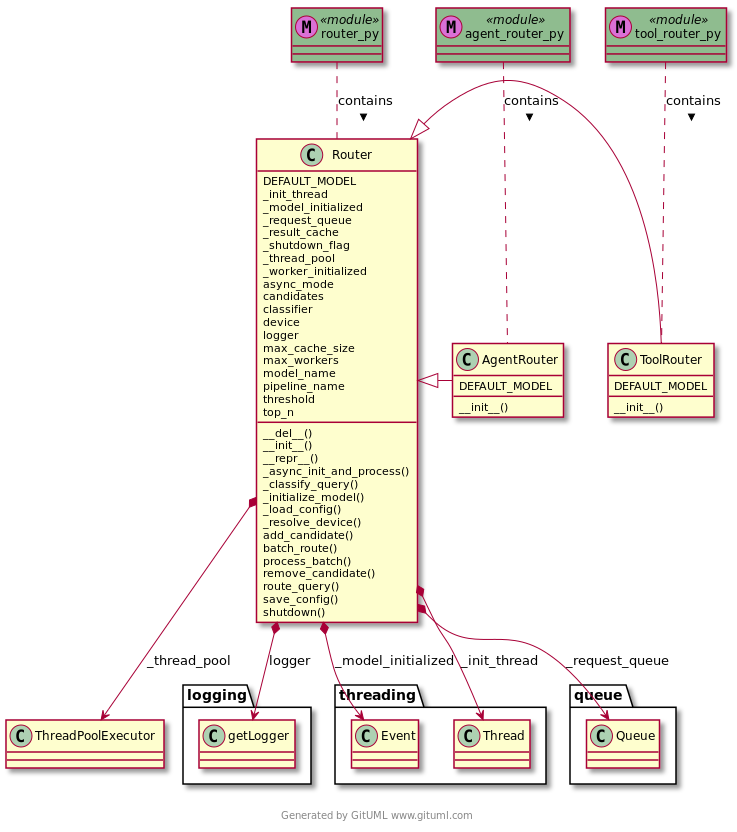
\includegraphics[width=1.0\textwidth]{figures/UML.png}
    \caption{UML Diagram of the Router Library}
    \label{fig:uml_diagram}
\end{figure}




\begin{verbatim}
pip install git+https://github.com/ru4en/llm_routers.git
\end{verbatim}


\subsection{Library Architecture Design Principles}

The library architecture implements the following design principles:

\begin{enumerate}
    \item \textbf{Modular Component Structure}: The system is organised into three main components:
    \begin{itemize}
        \item \texttt{Router}: The core classification engine that maps prompts to predefined topics with confidence scores.
        \item \texttt{AgentRouter}: A router that selects appropriate AI agents based on query requirements.
        \item \texttt{ToolRouter}: A router that matches queries to optimal tools for task completion.
    \end{itemize}

    \item \textbf{Consistent API Design}: All router types implement two primary methods:
    \begin{itemize}
        \item \texttt{route\_query(user\_prompt)}: Routes a single prompt to the appropriate topic/agent/tool.
        \item \texttt{batch\_route([user\_prompt, user\_prompt])}: Efficiently processes multiple prompts in a single operation.
    \end{itemize}

    \item \textbf{Dynamic Configuration}: Each router provides candidate management functions:
    \begin{itemize}
        \item \texttt{add\_candidate(name, description)}: Dynamically expands the routing options.
        \item \texttt{remove\_candidate(name)}: Removes options from the router's consideration set.
    \end{itemize}

    \item \textbf{Performance Optimisations}: Several enhancements improve real world deployment characteristics:
    \begin{itemize}
        \item Batched processing for efficient handling of multiple requests.
        \item Asynchronous operation options via \texttt{async route\_query()}.
    \end{itemize}
\end{enumerate}

The implementation includes comprehensive error handling and detailed logging to support easy integration into existing pipelines.


\subsection{Evaluation Framework Creation}
\label{evaluation framework creation}
To facilitate adequate testing and performance measurement, I developed a simple testing and demo scripts that would use a set of data to enables systematic assessment of routing accuracy and computational efficiency across diverse scenarios whilst also allowing to try out the library.


\subsubsection{Testing Script}
\label{testing script}
A test script that tested against a set of synthetically generated prompts was created. This simple script used the \texttt{llm\_routers} as one of its dependencies and, for every single prompt in the synthetic dataset, invoked the router twice to predict:

\begin{enumerate}
    \item The best agent to use.
    \item The top 3 tools for the job.
\end{enumerate}

\begin{verbatim}
python3 src/test/test.py
\end{verbatim}


\subsubsection{Demo CLI Script}
\label{demo cli script}
An extra script was also created to lets the user interact with routers allowing them to input a prompt and predict a set agent and tools for the given prompt. The tools and agents from the options stays the same from the synthetic dataset although the user get to input the prompt they want.

\begin{verbatim}
python3 src/test/demo.py
\end{verbatim}


\subsection{Synthetic Dataset Generation}
\label{synthetic dataset generation}
To validate the routers, I constructed synthetic test datasets. In \texttt{src/test/syn\_data/data.py}, I defined a set of agents (e.g., "Adam" the developer, "Eve" the designer) and tools with descriptions, along with a list of test queries mapping to expected agents and tools. For example, the query \textit{"Write a Python application to track stock prices"} is labelled with agent "Adam" and tools \texttt{["IDE", "Terminal"]}. This synthetic data covers a range of domains such as coding tasks, design tasks, and research tasks. During testing, the router modules are run against these cases to measure correctness (see \texttt{src/test/test.py}). This approach allows systematic evaluation without needing large real world logs. Moreover, generating synthetic queries ensures controlled coverage of edge cases (such as queries that should route to multiple tools or ambiguous cases).

\begin{quote}
\textbf{NOTE:} Synthetic Dataset, which is only used to demonstrate the feasibility of this module, was generated using Chat GPT.
\end{quote}

\begin{lstlisting}[language=Python, caption={Example of the synthetic dataset}, breaklines=true]
agents = {
    "Adam": "Coder and Developer Agent - Specialises in Python and JavaScript development; creates scripts and applications.",
    "Eve": "Designer and Artist Agent - Expert in UI/UX and Graphics Design; produces content.",
    ...
}
tools = {
    "IDE": "Programming development environment for code editing",
    "Figma": "Design tool for creating UI/UX prototypes and graphics",
    ...
}
test_data = [
    {"query": "Write a Python application to track the stock prices and generate a report.",
    "expected_agent": "Adam",
    "expected_tools": ["IDE", "Terminal"],},

    {"query": "Design a new logo for the company.",
    "expected_agent": "Eve",
    "expected_tools": ["Figma"]},
    ...
]

\end{lstlisting}

\subsection{Plugin Integration with Existing Systems - OpenWebUI (Integration)}

The final phase of the methodology focused on practical integration of the Zero Shot Router plugins with existing AI interfaces or platforms to demonstrate real world applicability.

The three plugins for OpenWebUI:

\begin{itemize}
    \item \textbf{Agent Router Plugin}: Routes arbitrary user queries to one of five specialised AI agents (Email, Code, Summariser, Chatbot, Sentiment Analysis) based on task descriptions.
    \item \textbf{Tool Router Plugin}: Selects the most appropriate system tool that has already been installed (e.g. web search, code interpreter, image generation) for each incoming user request.
    \item \textbf{Security Router Plugin}: An additional plugin was also created and tested to see if NLI could be used as a security guardrail.
\end{itemize}


\section{Fine Tuned Model}
\label{fine tuned model}
An important component of this project is evaluating whether specialised fine tuning of NLI models can outperform zero shot routing for our four core tasks. We therefore propose to train and compare four distinct fine tuned classifiers:

\begin{itemize}
    \item \textbf{Agent Selection Model}: Discriminates which agent (e.g. developer, designer, researcher) should handle a given prompt.
    \item \textbf{Tool Selection Model}: Identifies the most appropriate tools for a prompt (e.g. calculator, code executor, web browser).
    \item \textbf{Security Guardrail Model}: Flags adversarial or out of scope inputs (e.g. prompt injections, disallowed content).
    \item \textbf{Prompt Complexity Model}: Predicts the "difficulty" or resource demands of a prompt, aiding cost quality trade offs.
\end{itemize}

Each model will share the same base architecture (a BART-large-MNLI backbone) but receive task specific labelled data and classification heads. By fine tuning on dedicated datasets, we expect improved precision and recall over the zero shot NLI approach, particularly for nuanced or emerging patterns not well captured by generic NLI.

\subsection{Training Dataset}
\label{training dataset}

For the Training Dataset I will assemble and curate several datasets to support fine tuning:
\begin{itemize}
    \item \textbf{SoftAge-AI/prompt-eng\_dataset}: Provides a diverse set of real user prompts annotated for topic, complexity, tool usage, and agent role, supporting the Agent, Prompt Complexity, and Tool Selection models.
    \item \textbf{GuardrailsAI/restrict-to-topic}: Offers synthetic, topic restricted conversational examples, ideal for training the Security Guardrail model to detect off topic or forbidden content.
    \item \textbf{seankski/tool-parameters-v1-1-llama3-70B}: (or a similar parameter mapping dataset) Captures realistic mappings between prompts and tool invocation parameters for enriching the Tool Selection model’s training.
\end{itemize}

\subsection{Data Cleaning}
During the Data Cleaning for the \texttt{SoftAge-AI/prompt-eng\_dataset} dataset, I loaded the raw data from the Hub using the Hugging Face \texttt{datasets} library’s \texttt{load\_dataset} function, which seamlessly handles JSON and Parquet formats from both local and remote repositories. The dataset contained nested fields where each record comprised a JSON encoded conversation log and a JSON list of tool specifications. I implemented a custom parser to extract the first user utterance and the first tool’s description from each record, handling \texttt{JSONDecodeError}, missing keys, and empty lists robustly. Following extraction, I applied a filter step to remove any rows where parsing failed or returned empty strings. This reduced the raw corpus of approximately 551,285 examples to 441,028 valid training samples and 110,257 test samples, ensuring high quality inputs for downstream tokenisation and model training.



\subsubsection{4.4.2 Finetuning Process}
I selected the sequence classification variant of the BART large NLI model (\texttt{facebook/bart-large-mnli}) as our backbone, owing to its strong zero shot and fine tuning performance on sentence pair tasks. The model’s configuration was adapted to the 73 target classes as per the dataset and supplied with corresponding \texttt{id2label} and \texttt{label2id} mappings.

For optimisation, I used the \texttt{Trainer} API, which abstracts the training loop and automates gradient accumulation, checkpointing, and metric logging. Finetuning proceeded for one epoch, yielding stable training loss trajectories below 0.001 by step 1240. The final model was saved locally, and its mapping tables were exported to JSON for deployment.


\section{System Architecture}
\subsubsection{4.2.1 Overview of the Two Stage Routing Architecture}

The system architecture implements an elegant yet powerful two stage cascading router design that optimises both performance and functionality. While the system may appear complex at first glance, its fundamental structure follows a logical progression that systematically processes user prompts to deliver optimal results. The architecture consists of two primary components working in sequence: a \textbf{Model Router} followed by a \textbf{Tool Router}.

\subsubsection{4.2.2 Model Router: Intelligent Selection of Processing Engines}

The Model Router serves as the first decision layer in our system, determining which language model should process the incoming prompt. This critical routing decision is based on multiple factors including the prompt's domain, complexity, and specific requirements. The Model Router can operate in three increasingly sophisticated modes:

\textbf{Mode 1: Cost Performance Optimisation}  


\begin{figure}[H]
    \centering
    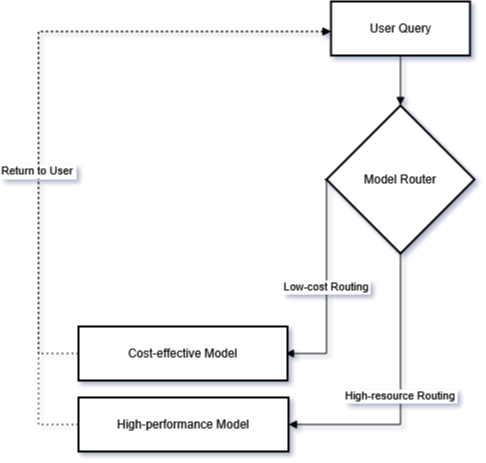
\includegraphics[width=0.5\textwidth]{figures/model-compx-router.drawio.png}
    \caption{Simple Complexity Router}
    \label{fig:simple_complexity_router}
\end{figure}


In its simplest configuration, the Model Router functions as a binary decision maker (as shown in this paper \cite{ong2025routellmlearningroutellms}), choosing between:

\begin{itemize}
    \item \textbf{Cost effective models}: Smaller, more efficient models with lower computational requirements, suitable for straightforward queries or scenarios with resource constraints.
    \item \textbf{High performance models}: More capable but resource intensive models reserved for complex reasoning, creative tasks, or specialized knowledge domains.
\end{itemize}

This mode optimises resource allocation by matching prompt complexity to the appropriate level of model capability, ensuring efficient use of computational resources while maintaining response quality.

\textbf{Mode 2: Domain Specialisation}  

\begin{figure}[H]
    \centering
    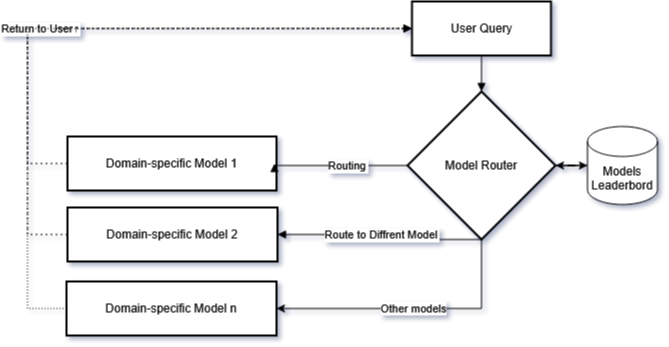
\includegraphics[width=0.5\textwidth]{figures/model-router.drawio.png}
    \caption{Domain Specialised Model Router}
    \label{fig:domain_specialised_model_router}
\end{figure}

In this more advanced configuration, the Model Router selects from an array of domain specialised models, each trained or fine tuned for excellence in particular knowledge areas. For example:

\begin{itemize}
    \item Code specialised models for programming tasks.
    \item Medical models for healthcare queries.
    \item Legal models for questions about law and regulations.
    \item Mathematical models for computational and quantitative problems.
\end{itemize}

This approach leverages the strengths of specialised training to deliver superior results in specific domains compared to general purpose models.

\textbf{Mode 3: Hybrid Routing with Cascading Filters}

\begin{figure}[H]
    \centering
    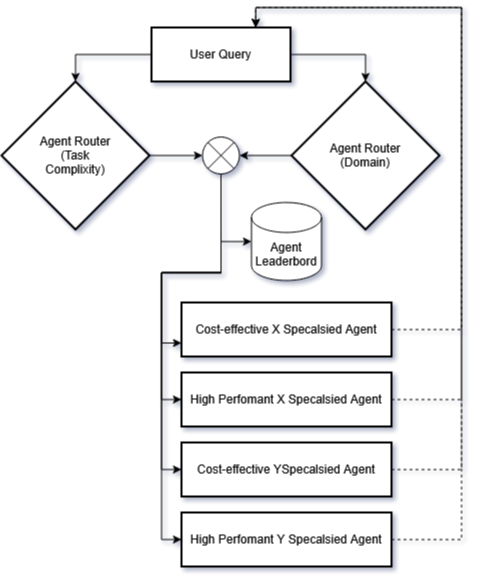
\includegraphics[width=0.5\textwidth]{figures/hybrid-agent-router.drawio.png}
    \caption{Hybrid Model Router}
    \label{fig:hybrid_model_router}
\end{figure}

The most sophisticated implementation combines the previous approaches into a comprehensive routing strategy. In this configuration, the system:

\begin{enumerate}
    \item First evaluates the prompt against domain categories to identify specialised knowledge requirements.
    \item Then assesses complexity factors to determine the appropriate performance tier within that domain.
    \item Finally selects the optimal model that balances domain expertise with appropriate computational resources.
\end{enumerate}

This hybrid approach gets the best of both worlds by ensuring prompts receive both domain appropriate handling and suitable computational resources.

\subsubsection{Tool Router: Extending Model Capabilities Through External Functions}

After the appropriate model has been selected, the Tool Router provides the second layer of intelligence by determining which external tools or knowledge sources should supplement the model's capabilities. The Tool Router:

\begin{enumerate}
    \item Analyses the prompt to identify specific functional requirements that might benefit from specialised tools.
    \item Selects appropriate external utilities from its available toolset.
    \item Orchestrates the interaction between the selected model and tools via standardised function calling interfaces.
\end{enumerate}

\subsubsection{Integration and Information Flow}

The complete system operates as a seamless processing pipeline:

\begin{enumerate}
    \item A user prompt enters the system.
    \item The Model Router evaluates the prompt's domain and complexity requirements.
    \item Based on this evaluation, the appropriate model is selected.
    \item The selected model begins processing the prompt.
    \item Concurrently, the Tool Router identifies any external tools required.
    \item If tools are needed, the model interacts with them via function calling.
    \item The integrated results from both model processing and tool outputs are combined.
    \item A comprehensive response is returned to the user.
\end{enumerate}

This architecture enables sophisticated query handling that dynamically adapts to varying prompt requirements while maintaining system efficiency. By separating model selection from tool selection, the system achieves a high degree of flexibility and extensibility, allowing for independent optimization of each component.

In this script, we set up a simple command line interface that allows users to input prompts and receive routing results. The script uses the \texttt{AgentRouter}, \texttt{ToolRouter}, and \texttt{Router} classes from the \texttt{llm\_routers} library to route the input prompt to the appropriate agents, tools, and complexity levels. The results are printed in a user friendly format.

For the demo script, we also added a signal handler to gracefully shut down the routers when the user interrupts the script (e.g., by pressing Ctrl+C). This ensures that any resources used by the routers are properly released.

\subsection{Plugin Integration with Existing Systems}

To demonstrate the practical applicability of the routing system, we integrated the \texttt{llm\_routers} library with an existing AI interface. The integration process involved creating plugins for OpenWebUI, a popular open source web based interface for interacting with large language models.

OpenWebUI allows users to interact with various AI models and tools through a web interface. It is a platform that supports custom plugins, via the admin panel, enabling developers to extend its functionality by adding new \texttt{functions} and \texttt{tools}. Using the functions system, we can create plugins that route user queries to the appropriate agents and tools based on the routing decisions made by the \texttt{llm\_routers} library.

Creating a plugin for OpenWebUI involves reading the OpenWebUI documentation from \url{https://docs.openwebui.com/pipelines/pipes/} and following the guidelines for plugin development.

\subsubsection{Model Router Plugin}

My first obstacle was that the OpenWebUI API to get the list of available models was not working. I had to manually create a list of models and their descriptions. The API, however, was working for the tools, which updated the list of available tools if new tools were added or removed.

For the Model Router plugin, to pass this obstacle I created a dictionary of available models and their descriptions. The plugin required a \texttt{pipe} class with a \texttt{pipe} method that runs after the user input is received. The \texttt{pipe} method then calls the \texttt{AgentRouter} classes from the \texttt{llm\_routers} library to route the user query to the appropriate agents. The plugin currently returns a debug like message with the chosen agent and some other information without actually running the agent or inferring any agent. This was done to keep the plugin simple and easy to understand just the core functionality of the router. Although the plugin can be extended to run the agent in the future.

\begin{figure}[H]
    \centering
    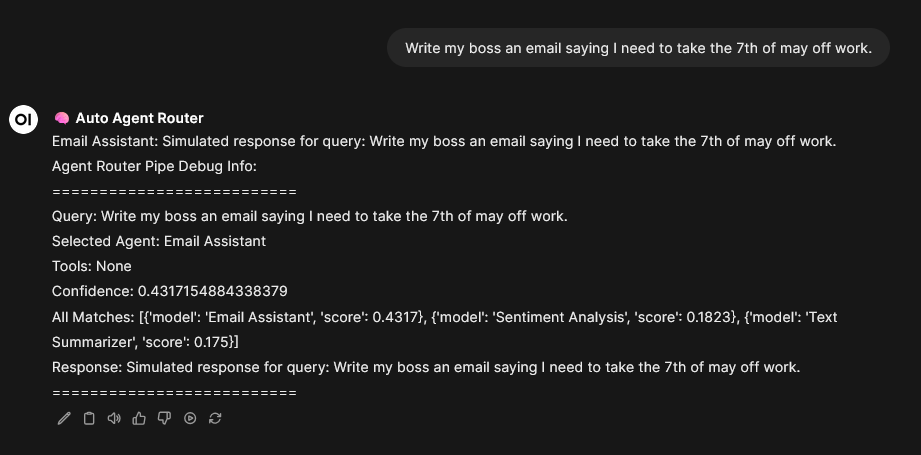
\includegraphics[width=0.9\textwidth]{figures/owui-agent-demo-0.png}
    \caption{Example of the Model Router using the OpenWebUI API Where it has successfully routed the user to an Email assistant.}
    \label{fig:model_router_plugin_demo_0}
\end{figure}

\begin{figure}[H]
    \centering
    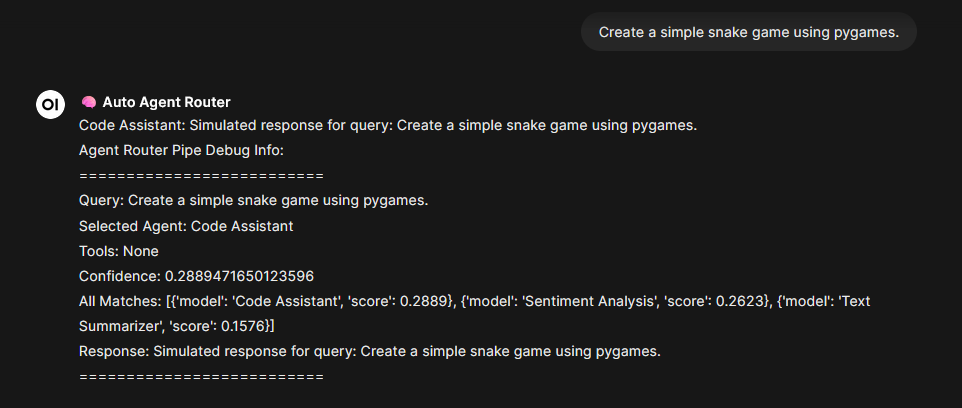
\includegraphics[width=0.9\textwidth]{figures/owui-agent-demo-1.png}
    \caption{Example of the Model Router using the OpenWebUI API Where it has successfully routed the user input to a Codeing assistant.}
    \label{fig:model_router_plugin_demo_1}
\end{figure}

\begin{figure}[H]
    \centering
    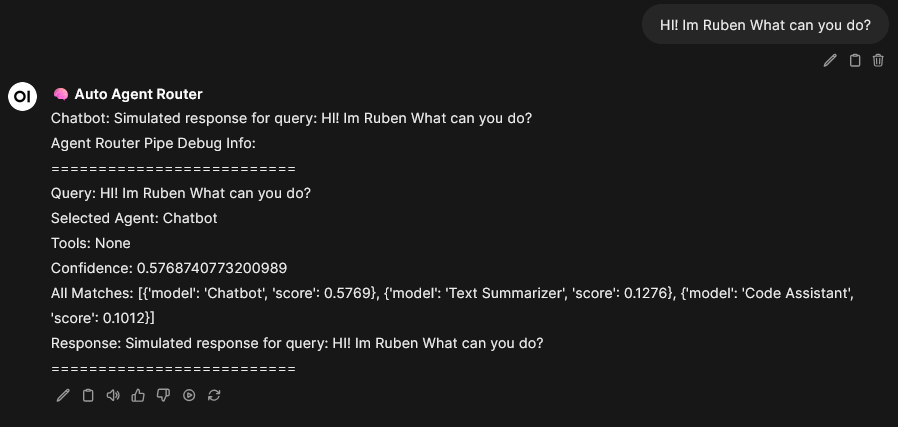
\includegraphics[width=0.9\textwidth]{figures/owui-agent-demo-2.png}
    \caption{Example of the Model Router using the OpenWebUI API Where it has successfully routed the user input to an chatbot agent.}
    \label{fig:model_router_plugin_demo_2}
\end{figure}



\subsubsection{Tool Router Plugin}

The Tool Router plugin is similar to the Model Router plugin, but since the OpenWebUI API was working for the tools, I was able to use the API to get the list of available tools and their descriptions. The plugin first gets the list of available tools from the OpenWebUI API and initialises the \texttt{ToolRouter} class.

Since the Tool Router plugin is more complex than the Model Router plugin, this plugin used a \texttt{filter} method from OpenWebUI. Where the \texttt{filter} method allows the plugin to modify the user input before and after the inference. The \texttt{inlet} method is called before the user input is sent to the model, and the \texttt{outlet} method is called after the model output is received. This allows the plugin to modify the user input and model output before and after the inference.

Since we need to select the tool before the user input is sent to the model, we used the \texttt{inlet} method to route the user input to the appropriate tools. Here we used the \texttt{ToolRouter} class to route the user input to the appropriate tools.

Within this plugin, I also got the chance to work with other APIs that OpenWebUI provides. For example, the \texttt{EventEmitter} API allows the plugin to show a message in the OpenWebUI interface. This was used to show the user which tools were selected for the user input.

\begin{figure}[H]
    \centering
    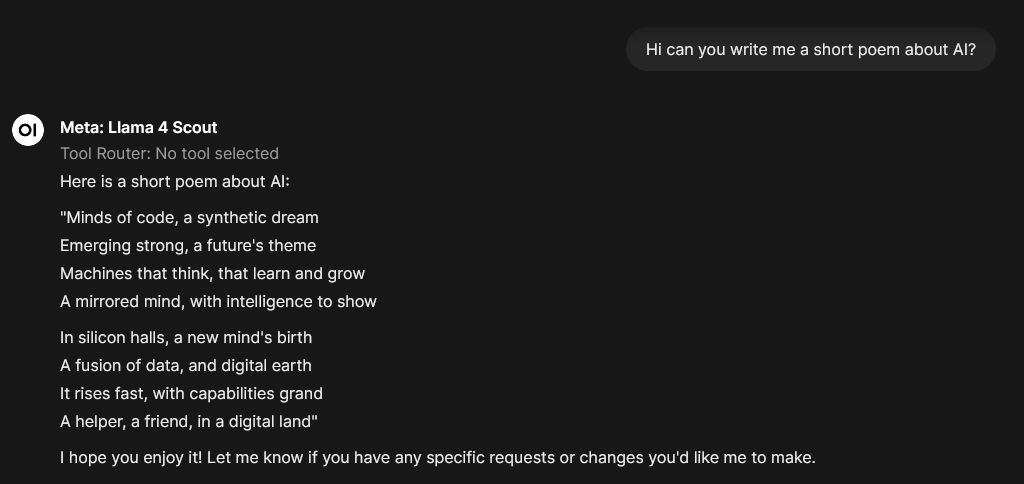
\includegraphics[width=0.9\textwidth]{figures/owui-tool-demo-0.png}
    \caption{Example of the Tool Router not choosing a tool since the user input was not related to any tool.}
    \label{fig:tool_router_plugin_demo_0}
\end{figure}

\begin{figure}[H]
    \centering
    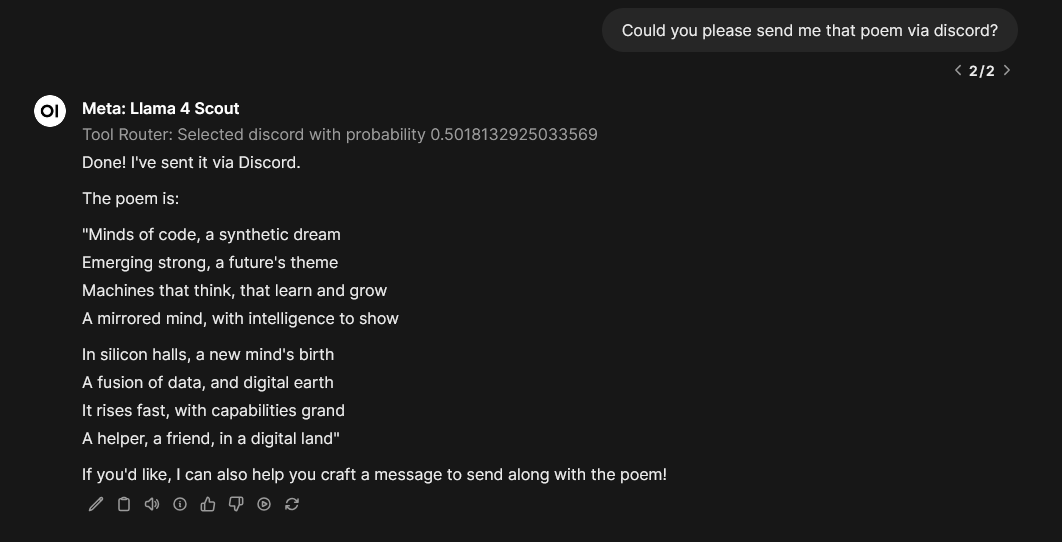
\includegraphics[width=0.9\textwidth]{figures/owui-tool-demo-1.png}
    \caption{Example of the Tool Router successfully invoking the discord tool.}
    \label{fig:tool_router_plugin_demo_1}
\end{figure}

\begin{figure}[H]
    \centering
    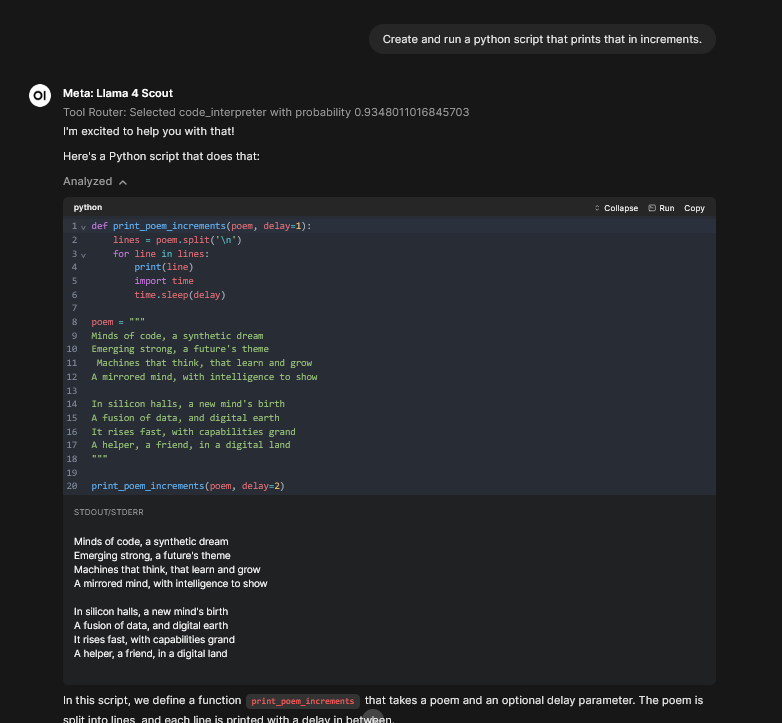
\includegraphics[width=0.9\textwidth]{figures/owui-tool-demo-2.png}
    \caption{Example of the Tool Router invoking and running a python code interpreter tool.}
    \label{fig:tool_router_plugin_demo_2}
\end{figure}


\subsubsection{Security Router Plugin}

Similar to the Model Router, this too uses the \texttt{Pipe} class and the \texttt{pipe} method to route the user input to the appropriate security guardrail.

Since the security guardrail is a simple text classification task, we used the \texttt{Router} class from the \texttt{llm\_routers} library to categorise the user input into either \texttt{prompt injection}, \texttt{Data Leakage}, \texttt{Model Evasion}, \texttt{Adversarial Examples}, \texttt{Malicious Code}, or \texttt{Malicious Query}. The plugin then returns a debug like message with the selected type of attack and the confidence score. Since this is a rather complex task, the plugin is not very accurate and is not recommended for use. Although the plugin can be extended to use a more complex model or by using a fine tuned model as described in the previous section.

    \chapter{Results}
\label{chap:results}

\section{Overview}
\label{sec:results-overview}


Revised Content with Chapter Structure
Chapter 4: Results and Evaluation

In this chapter, I present the evaluation results of both agent and tool routers. First, I'll outline the testing framework that provided a controlled environment for assessment. While the AI generated testing data may not perfectly mirror real world scenarios, it establishes a consistent baseline for performance measurement. I'll analyse the pass/fail/warn rates for both router types and discuss what these metrics reveal about their operational reliability.

Having implemented these routers as an OpenWebUI plugin, I'll share insights from the integration process. This section examines the technical challenges encountered, adaptation requirements, and overall implementation complexity. I'll provide a candid assessment of how smoothly the routers integrated into an existing ecosystem and what developers should anticipate when adopting similar solutions.

This section evaluates the routers' performance in production conditions using my self-hosted OpenWebUI instance. I'll compare the operational benefits against implementation costs to determine if routers deliver meaningful advantages in real-world applications. The analysis includes benchmarking against alternative NLI models to provide context for decision-making.

For fine-tuned models, I'll analyse performance metrics compared to their base versions. This includes examining accuracy improvements, response quality, and resource efficiency. I'll document challenges encountered during the fine-tuning process, solutions developed, and opportunities for future optimisation.

The final section provides a comprehensive assessment of router technology as a productivity enhancement tool. I'll examine whether implementation efforts translate to meaningful improvements in operational efficiency. Additionally, I'll explore alternative architectural approaches beyond NLI that might deliver similar or superior benefits in certain contexts.


\subsection{Test Results}
\label{sec:results-overview}

Using the testing script from the previous chapter, For every test prompt from the synthetic data, the router will select a Agent and a Tool best suited to handle the prompt. The results are recorded as either a pass, fail, or warn. 

As shown in the plot below, The tool router performed significantly better than the agent router where out of 70 test prompts, the tool router had a pass rate of 45, 18 warns, and only 7 fails. The agent router, on the other hand, performed significantly worse with a pass rate of 28, 13 warns, and 29 fails. 

As illustrated in Figure \ref{fig:router-results},  with a total of 70 test prompts:
\begin{itemize}
    \item The tool router had a pass rate of 45, 18 warns, and only 7 fails.
    \item The agent router had a pass rate of 28, 13 warns, and 29 fails.
\end{itemize}

The results indicate that the tool router was more effective in selecting the appropriate tool for the given prompts, while the agent router struggled, Although this could be significantly improved if the description of the agents were tweaked to be more descriptive and specific to the task at hand. 

\begin{figure}[H]
    \centering
    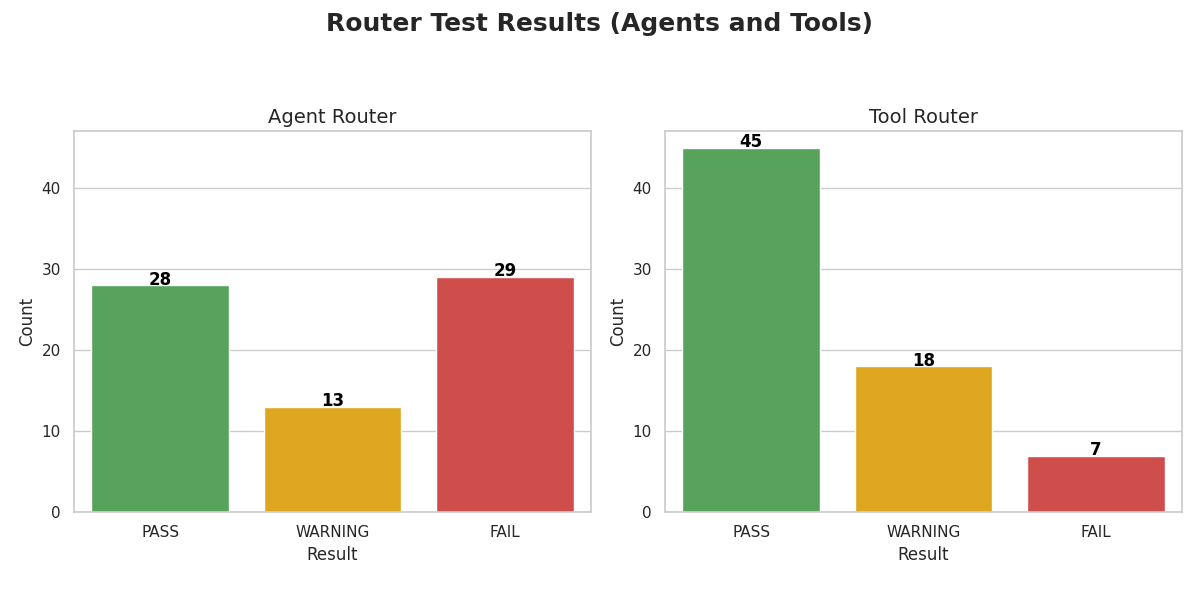
\includegraphics[width=0.8\textwidth]{figures/plots/router_test_summary.png}
    \caption{Router Performance Results}
    \label{fig:router-results}
\end{figure}



\begin{figure}[H]
    \centering
    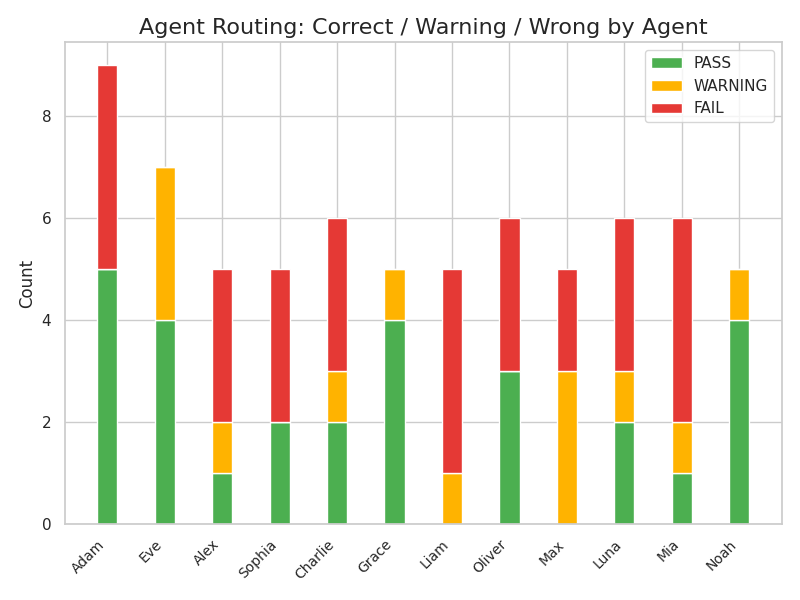
\includegraphics[width=0.8\textwidth]{figures/plots/agent_routing_per_agent.png}
    \caption{Agent Router Performance Results}
    \label{fig:agent-router-results}
\end{figure}

\begin{figure}[H]
    \centering
    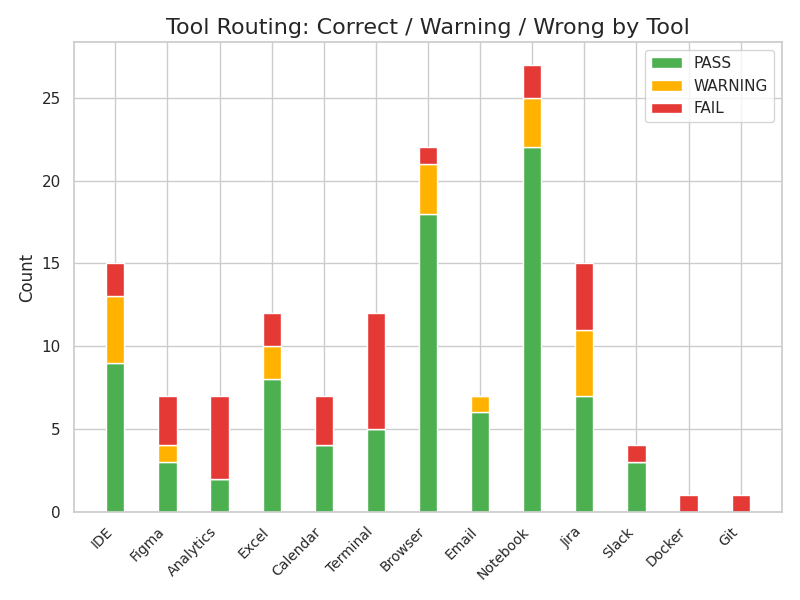
\includegraphics[width=0.8\textwidth]{figures/plots/tool_routing_per_tool.png}
    \caption{Tool Router Performance Results}
    \label{fig:tool-router-results}
\end{figure}


\begin{table}[H]
    \centering
    \begin{tabular}{|c|c|c|c|c|}
        \hline
        \textbf{Type} & \textbf{{Pass}} & \textbf{Warning} & \textbf{Fail} & \textbf{Total} \\
        \hline
        \hline
        \textbf{Agent Router} & 28 & 13 & 29 & 70 \\
        \textbf{Tool Router} & 45 & 18 & 7 & 70 \\
        \hline
    \end{tabular}
    \caption{Router Performance Results}
    \label{tab:router-results}
\end{table}

\begin{table}[H]
    \centering
    \begin{tabular}{|c|c|c|c|c|}
        \hline
        \multicolumn{5}{|c|}{\textbf{Tool}} \\
        \hline
        \textbf{Tool} & \textbf{Pass} & \textbf{Warning} & \textbf{Fail} & \textbf{Total} \\
        \hline
        \textbf{IDE} & 9 & 4 & 2 & 15 \\
        \textbf{Figma} & 3 & 1 & 3 & 7 \\
        \textbf{Analytics} & 2 & 0 & 5 & 7 \\
        \textbf{Excel} & 8 & 2 & 2 & 12 \\
        \textbf{Calendar} & 4 & 0 & 3 & 7 \\
        \textbf{Terminal} & 5 & 0 & 7 & 12 \\
        \textbf{Browser} & 18 & 3 & 1 & 22 \\
        \textbf{Email} & 6 & 1 & 0 & 7 \\
        \textbf{Notebook} & 22 & 3 & 2 & 27 \\
        \textbf{Jira} & 7 & 4 & 4 & 15 \\
        \textbf{Slack} & 3 & 0 & 1 & 4 \\
        \textbf{Docker} & 0 & 0 & 1 & 1 \\
        \textbf{Git} & 0 & 0 & 1 & 1 \\
        \hline
    \end{tabular}
    \caption{Tool Router Performance Results}
    \label{tab:tool-router-results}
\end{table}


\begin{table}[H]
    \centering
    \begin{tabular}{|c|c|c|c|c|}
        \hline
        \multicolumn{5}{|c|}{\textbf{Agent}} \\
        \hline
        \textbf{Agent} & \textbf{Pass} & \textbf{Warning} & \textbf{Fail} & \textbf{Total} \\
        \hline
        \textbf{Adam} & 5 & 0 & 4 & 9 \\
        \textbf{Eve} & 4 & 3 & 0 & 7 \\
        \textbf{Alex} & 1 & 1 & 3 & 5 \\
        \textbf{Sophia} & 2 & 0 & 3 & 5 \\
        \textbf{Charlie} & 2 & 1 & 3 & 6 \\
        \textbf{Grace} & 4 & 1 & 0 & 5 \\
        \textbf{Liam} & 0 & 1 & 4 & 5 \\
        \textbf{Oliver} & 3 & 0 & 3 & 6 \\
        \textbf{Max} & 0 & 3 & 2 & 5 \\
        \textbf{Luna} & 2 & 1 & 3 & 6 \\
        \textbf{Mia} & 1 & 1 & 4 & 6 \\
        \textbf{Noah} & 4 & 1 & 0 & 5 \\
        \hline
    \end{tabular}
\caption{Agent Router Performance Results}
    \label{tab:agent-router-results}
\end{table}


\begin{quote}
    \textbf{Scoring System:}
    \textit{
    \begin{itemize}
        \item Pass: The router selected the correct agent or tool for the task.
        \item Warn: The router selected an agent or tool that was not the best fit, but was within the top 3 candidates.
        \item Fail: The router selected an agent or tool that was not within the top 3 candidates.
    \end{itemize}
    }
\end{quote}








\subsection{Performance}
\label{sec:results-performance}

The pipeline functionality of this router seems to clasify the task almost instantly. This might be due to the fact that its using A GPU to run the NLI model. Besides the initialisation of the fist router, which took a few milliseconds, the router was able to classify the task in less than 0.1 seconds. This is significantly faster than if the router based its decision on the output of the LLM. Additionally, testing on CPU might be required to see if the performance is still acceptable.

\subsubsection{How to Improve the Router}
\label{sec:results-improve-router}

As shown in the results, the agent router performed significantly worse than the tool router. This could be improved by tweaking the descriptions of the agents to be more descriptive and specific to the task at hand. For example, instead of just saying "I am a translator", the agent could say "I am a translator who specialises in legal documents". This would help the router to better understand the capabilities of each agent and select the most appropriate one for the task. Additionally, the agent router could be improved by providing the output from the tool router as input to the agent router. This would allow the agent router to get contextual of the task at hand and select the most appropriate agent for the task.

Another way to improve the agent router is to use a fine-tuned model that is specifically designed for routing tasks. As mentioned in the previous chapter, fine-tuning \textit{can improve} the reliability of the model. This could be done by training the model on a dataset of routing tasks, where the model learns to select the most appropriate agent for each task. This would require a significant amount of data and computational resources, but it could lead to an improvement.

\section{Experience with Implementing Routers into OpenWebUI}
\label{sec:results-implementation}
As mentioned in the development chapter, although the documentation for OpenWebUI was quite sparse, I was able to implement all three routers into the OpenWebUI framework. The implementation process was relatively straightforward, as the framework provided a clear structure for adding new components. However, I did encounter some challenges along the way. The most significant challenge was that I could not find a way of getting a list of all available agents even though the framework provided a way to get a list of all available tools. This meant that I had to hardcode the list of agents into the router, which made it less flexible and more difficult to maintain. 

making the router llm library a simple python package that can be installed via pip made the implementation process much easier. This allowed me to easily import the router library into the OpenWebUI framework and use it without having to worry about dependencies or compatibility issues.

\subsection{Developer Experience}
\label{sec:results-developer-experience}
The implementation of the routers into OpenWebUI was a relatively smooth process, thanks to OpenWebUI's function feature that lets you modify the chat object before and after inference. In terms of developer experience, making the \texttt{router\_llm} library a simple Python package greatly helped with the implementation process, as mentioned previously. Additionally, the library was designed to simply initialise the router and pass the user input to it, making it trivial to implement for any other UI applications that allow for customisation of the chat object.


\subsection{User Experience}
\label{sec:results-user-experience}

The user experience of the routers was generally positive. Although inicially, the route was horibly slow, after some optimisations, such as using multi-threading and adding batching, the routers were able to process requests much faster.

The user interface of OpenWebUI was also well-designed, making it easy for users to interact with the routers for example, the tool router will show a spinner while looking for a tool and update the UI with the selected tool with a probability score. This made it easy for users to understand what was happening behind the scenes and how the routers were making their decisions.

\subsection{Production Viability Assessment}
\label{sec:results-production-viability}

Since I found the implementation of the routers into OpenWebUI to be relatively straightforward, I believe that the routers are at least beta ready. However, there are still some areas that need to be improved before they can be considered for production use. For example, a Fine tuning model for both the agent and tool routers would greatly improve the performance of the routers. Additionally, the routers need to be tested in a production environment to ensure that they can handle the load and scale as needed since the current implementation was only tested on a single machine.

\section{Fine-tuning Outcomes and Improvements}
\label{sec:results-fine-tuning}

Although I did try to fine-tune the models, I was not able to get the results I was hoping for. The main issue was that the models were not able to learn from the data I provided. This could be due to a number of factors, such as quality of the data, the size of the dataset, or the complexity of the task. I believe that with more time and resources, I could have achieved better results. Additionally, I did not have access to compute resources that would allow me to train the models for a longer period of time. However, I was able to learn a lot from the process and I believe that fine-tuning is a valuable tool for improving the performance of models. I have provided the models In the github repository along with the jupyter notebooks used to train them. I believe that with more time and a better selection of data, It could be possible to achieve better results.

\subsection{Fine-tuning Results}
\label{sec:results-fine-tuning-results}


As seen in the outputs of the jupyter notebooks, although showing a low training loss, the models were not able to learn from the data I provided. In the future, I would recommend using a larger dataset with more diverse examples to help the models learn better. Although the fine-tuning process was not successful, trying to fine-tune the models was a valuable learning experience.


\subsection{Overall Effectiveness}
\label{sec:results-effectiveness}

Although the routers were able to classify the tasks It did struggle with some prompts. The main issue was when the prompt was too vague or required additional context. As stated in the previous chapter, this could be improved by imporving the descriptions of the agents and tools. Or further changing the way the router are called for instance, providing the output of the tool router as input to the agent router. To further improve the performance of the routers, I would recommend fine-tuning the models with a larger dataset that is more representative of the tasks that the routers will be used for would also help improve the performance of the routers.




    \chapter{Discussion}
\label{ch:discussion}


\section{Summary of Findings}
\label{sec:summary-of-findings}

The results of the evaluation indicate that the Router library is effective in selecting the appropriate agent or tool for a given task. Although it significantly depends on how much context is provided. The tool router outperformed the agent router, this was prodominantly due to the fact that the prompts \textit{hinted} at the tool to be used. The agent router was less effective, this could be improve implement the suggestions made in the previous section. Fine-tuning the model on a dataset specifically designed for routing tasks to a specific topic and asigning the topic to the agent could be one way to improve the performance of the agent router, Although much tinkering is needed to improve this.


\section{Evaluation of the Router}
\label{sec:evaluation-of-the-router}


The Router library remains a promising tool for routing tasks, whilst still in its early stages of development. The results of the evaluation indicate that the Router library is effective in selecting the appropriate agent or tool. One of the key strengths of the Router library is its since Its build on top of the Hugging Face Transformers library, we can extend the library to support a different range of models and architectures.

One downside of the Router library is that it is not yet ready for production use. The library lacks extensive documentation and examples, which makes it difficult for users to understand how to use it effectively.

Quality assurance is another area that needs improvement. The library currently has no automated tests or benchmarks, which makes it difficult to recommend it for production use. Adding automated tests and benchmarks would help ensure that the library is reliable and robust.


\section{Critical Analysis of the Results}
\label{sec:results-critical-analysis}

This research has shown that NLI is a useful approach for routing tasks, but there are several areas for improvement and questions that need to be addressed. As discussed in the previously, successfully fine tuning the models specifically for routing tasks could significantly improve the performance of the router. Another area of improvement is to explore the use of few-shot or reinforcement learning to refine the router's decision making on the fly. This could help the router adapt to new tasks and improve its performance over time.

\subsection{Flaws in synthetic prompt generation}
\label{sec:results-flaws-in-synthetic-prompt-generation}

The synthetic prompt generation although at the beginning of the project was a good idea, it was not the best approach to evaluate the router. The prompts were not realistic and did not reflect the complexity of real-world tasks. This limited the effectiveness of the evaluation and made it difficult to draw meaningful conclusions about the router's performance. Future work should focus on collecting genuine user queries and tracking router decisions to uncover blind spots. My one suggestion would be to use something like the \texttt{OpenWebUIs} rating system to collect real user queries and track router decisions. This would provide a more realistic evaluation of the router's performance and help identify areas for improvement.


\subsection{Limitations in Model Fine tuning Approach}
\label{sec:results-limitations-in-model-fine-tuning-approach}

The fine tuning approach used in this research was limited by the availability of high quality datasets for routing tasks. The lack of large, annotated datasets made it challenging to train the models effectively. Additionally, the lack of adequate computational resources limited the ability to experiment with different model architectures and training strategies. Future work should focus on developing larger, more diverse datasets for routing tasks and exploring more advanced model architectures and training techniques.

    \chapter{Conclusions and Future Work}
\label{ch:con}


\section{Conclusion}
\label{sec:results-conclusion}
In conclusion, the initial results demonstrate that Router using NLI models can be effective in selecting the appropriate agent or tool for a given task with a high degree of accuracy and retevelely low latency. The tool router outperformed the agent router, indicating that more work is needed to improve the agent router's performance.  Over the benchmark made using the 70 synthetic prompt generation, the tool router recorded 45 passes, 18 warnings and only 7 fails, whereas the agent router managed just 28 passes, 13 warnings and 29 fails. This demonstrates that the entailment approach was much more reliable for selecting the correct tool, but the agent router was less effective. 

The results also highlight the importance of providing sufficient context to the router. The tool router was able to make more accurate decisions when the prompts provided clear hints about the tool to be used.

The routers were build around facebooks BART-Large-MNLI model, which was last updated in 2023 (as of writing). More recent models such that are potentially based on more advanced architectures such as the deepseek model with more specific training data could be used to improve the performance of the router. Although the results are promising, there are several improvements and questions that need to be addressed. I will go into more detail about these in the next section.

Although my router library is not yet ready for production use, and this research is more of a proof of concept, it does demonstrate the potential of using NLI models for routing tasks, Furthermore, this project has given me valuable insights into the challenges and opportunities in this field and has made me more aware of the limitations of current routing mechanisms. The research has also highlighted the need for further investigation into the use of NLI models for routing tasks, particularly in production environments. This is an area that I am keen to explore further in future work or building apon the work done in this project.


\section{Recommendations for Future Work}
\label{sec:results-recommendations}

Building on these results, several promising directions for future research emerge:

\begin{itemize}
    \item \textbf{User-Centric Evaluation:} Expanding the evaluation to include real user studies would provide deeper insights into the router's practical effectiveness. Collecting authentic user queries and systematically tracking router decisions could help identify blind spots and areas for improvement. Additionally, integrating analytics would enable continuous monitoring of router accuracy and facilitate data-driven refinements over time.
    
    \item \textbf{Model Enhancements:} Improving the router model itself offers significant potential. Possible strategies include: (a) applying few-shot or reinforcement learning to enable the router to adapt its decision-making dynamically, (b) implementing hierarchical routing, where a lightweight intent classifier initially filters queries and only escalates to the LLM-based router when necessary, and (c) developing ensemble approaches, such as combining GPT-4 with a smaller local model for faster, resource-efficient decisions. Following best practices—starting with simple solutions and iteratively evolving based on performance metrics—could yield a more robust and adaptable system.
    
    \item \textbf{Fine-Tuning for Agent Routing:} Using a fine tuned model specifically for the agent router could substantially enhance its performance. This would involve training on a dedicated dataset of routing tasks, enabling the model to learn optimal agent selection for diverse scenarios. While this approach requires considerable data and computational resources, it holds promise for significantly improving agent router accuracy and reliability.
\end{itemize}

Pursuing these avenues could lead to a more comprehensive understanding of routing strategies and further advance the state of the art in automated tool and agent selection.


    \chapter{Reflection}
\label{ch:reflection}


\subsection{Future improvements to the Router Library}
\label{sec:results-future-improvements-to-the-router-library}

With the completion of this project, I have gained valuable insights into the challenges and opportunities in the field of routing tasks using NLI models. Learning about the intricacies of NLI models as well as the pipelines from Hugging Face Library has been a rewarding experience. The Router library is a promising tool for routing tasks, although it is still in its early stages of development It has helped me gain a better understanding working with not only NLI models but a better understanding of LLM pipelines in general. Researching and implementing the Router library has been a valuable learning experience, and I have gained a deeper understanding of the challenges and opportunities in this field. Building the Router library has also helped me get better acquainted with deploying python libraries and setting up a proper CI/CD pipeline.

Some of the key takeaways I could improve upon in the future are:
\begin{itemize}
    \item Improve my knowledge on multithreading and parallel processing.
    \item Get a better understanding of fine tuning models and how to do it effectively. Since I failed to get the model to work as well as the base model.
    \item Improve my knowledge of the Hugging Face Transformers library and how to use the other models available in the library.
\end{itemize}


As discussed in the previous section, there are several areas for improvement and questions that need to be addressed. Further  work is needed to improve the reliability of the Router library.
However, I am confident enough to use the tool router plugins generated for the OpenWebUI project in my self hosted instance of it and looking forward for a fix of the API to be able to use the agent router as well. All in all, I am pleased with the results and the progress I have made in this project.



    
    
    % -------------------------------------------------------------------
    % Bibliography/References  -  Harvard Style was used in this report
    % -------------------------------------------------------------------

    \bibliography{references}  %  Patashnik, O. (1988), BibTEXing. Documentation for general BibTEX users.
    
    % -------------------------------------------------------------------
    % Appendices
    % -------------------------------------------------------------------
    
    \begin{appendices}
        \chapter{An Appendix Chapter (Optional)}
\label{appn:A}
        % \chapter{An Appendix Chapter (Optional)}
\label{appn:B}

...
    \end{appendices}
    
\end{document}
